% Module 1: Machine Learning - course project report
% Compile with XeLaTeX: latexmk -xelatex report.tex  (uses ctex + Fandol fonts shipped with TeX Live)
\documentclass{article}
\PassOptionsToPackage{numbers,compress}{natbib}
\usepackage[final]{template22}
% Common packages
\usepackage[utf8]{inputenc} % allow utf-8 input
\usepackage[T1]{fontenc}    % use 8-bit T1 fonts
\usepackage{microtype}
\usepackage{times}
\usepackage{graphicx}
\usepackage{amsmath,amssymb,mathbbol}
% \usepackage{algorithmic}
% \usepackage[linesnumbered,ruled,vlined]{algorithm2e}
\usepackage{acronym}
\usepackage{enumitem}
\usepackage[pagebackref=true,breaklinks=true,colorlinks]{hyperref}
\usepackage{balance}
\usepackage{xspace}
\usepackage{setspace}
\usepackage[skip=3pt,font=small]{subcaption}
\usepackage[skip=3pt,font=small]{caption}
\usepackage[dvipsnames]{xcolor}
\usepackage[capitalise]{cleveref}
\usepackage{booktabs,tabularx,colortbl,multirow,array,makecell}
% \usepackage{overpic,wrapfig}

\usepackage{fancyhdr}
\hypersetup{pdfencoding=auto,colorlinks=true,allcolors=black}
\renewcommand{\headrulewidth}{0.5pt}
\renewcommand{\footrulewidth}{0pt}
\fancyhf{}
\fancyhead[C]{}
\fancyhead[C]{}
\fancyfoot[C]{\thepage}

% Handy shorthand
\makeatletter
\DeclareRobustCommand\onedot{\futurelet\@let@token\@onedot}
\def\@onedot{\ifx\@let@token.\else.\null\fi\xspace}
\def\eg{\emph{e.g}\onedot} 
\def\Eg{\emph{E.g}\onedot}
\def\ie{\emph{i.e}\onedot} 
\def\Ie{\emph{I.e}\onedot}
\def\cf{\emph{c.f}\onedot} 
\def\Cf{\emph{C.f}\onedot}
\def\etc{\emph{etc}\onedot} 
\def\vs{\emph{vs}\onedot}
\def\wrt{w.r.t\onedot} 
\def\dof{d.o.f\onedot}
\def\etal{\emph{et al}\onedot}
\makeatother

\definecolor{gray}{gray}{0.9}

% Handy math ops
\DeclareMathOperator*{\argmax}{arg\,max}
\DeclareMathOperator*{\argmin}{arg\,min}
\newcommand{\norm}[1]{\left\Vert #1 \right\Vert}

% % Spacing
\frenchspacing
% \medmuskip=2mu   % reduce spacing around binary operators
% \thickmuskip=3mu % reduce spacing around relational operators
% \setlength{\abovedisplayskip}{3pt}
% \setlength{\belowdisplayskip}{3pt}
% \setlength{\abovecaptionskip}{3pt}
% \setlength{\belowcaptionskip}{3pt}
\setlength\floatsep{0.5\baselineskip plus 3pt minus 2pt}
\setlength\textfloatsep{0.5\baselineskip plus 3pt minus 2pt}
\setlength\dbltextfloatsep{0.5\baselineskip plus 3pt minus 2pt}
\setlength\intextsep{0.5\baselineskip plus 3pt minus 2pt}

\makeatletter
\renewcommand{\paragraph}{%
  \@startsection{paragraph}{4}%
  {\z@}{0ex \@plus 0ex \@minus 0ex}{-1em}%
  {\hskip\parindent\normalfont\normalsize\bfseries}%
}
\makeatother

% Graphics path
\graphicspath{{figures/}}

% Clever references
\crefname{algorithm}{Alg.}{Algs.}
\Crefname{algorithm}{Algorithm}{Algorithms}
\crefname{section}{Sec.}{Secs.}
\Crefname{section}{Section}{Sections}
\crefname{table}{Tab.}{Tabs.}
\Crefname{table}{Table}{Tables}
\crefname{figure}{Fig.}{Fig.}
\Crefname{figure}{Figure}{Figure}

% Acronym
\acrodef{pku}[PKU]{Peking University}
\usepackage[fontset=fandol]{ctex}

\title{CIFAR-10 Classification with SimpleCNN, SimpleViT and a CNN--ViT Composition}

\author{%
  雷源泽 \quad 2510124204\\
  Peking University
}

\begin{document}
\maketitle

\begin{abstract}
We implement a \emph{SimpleCNN} (85{,}642 parameters) and a from-scratch \emph{SimpleViT} in PyTorch and train both on CIFAR-10 for $75$ epochs with W\&B tracking. The CNN reaches \textbf{79.48\%} test accuracy and the ViT \textbf{65.01\%}. The optional \emph{SimpleComposition} ($81{,}194<120$K parameters) reaches \textbf{69.98\%}.
\end{abstract}

\section{Method}\label{sec:method}

\subsection{Data preparation}
\texttt{prepare\_data.py} loads the $50{,}000$-image CIFAR-10 training set and splits the official $10{,}000$-image test set into validation/test with an $8{:}2$ ratio using \texttt{random\_split} and a \texttt{torch.Generator} seeded with $0$ (reproducible). All images use \texttt{ToTensor()} and normalisation with mean/std $0.5$; training additionally uses \texttt{RandomCrop(32, padding=4)} and \texttt{RandomHorizontalFlip()}.

\subsection{SimpleCNN}
Two $3\times3$ convolutions ($32$/$64$ channels) with ReLU and $2\times2$ max-pooling (three pools in total: $32\!\to\!16\!\to\!8\!\to\!4$), flatten ($64\times4\times4=1024$), dropout, and two fully connected layers ($1024\!\to\!64\!\to\!10$). Parameter count: $896+18{,}496+65{,}600+650=85{,}642<100$K. Dropout is active in training and disabled by \texttt{model.eval()}. \texttt{forward\_map()} exposes the $4\times4$ feature map for the bonus model.

\subsection{SimpleViT}
All blocks are implemented from scratch (no \texttt{nn.Transformer*}): a \texttt{FeedForward} block (LayerNorm--Linear--GELU--Dropout--Linear--Dropout); multi-head \texttt{Attention} with a fused QKV projection, scaled dot-product attention ($1/\sqrt{d_{head}}$), softmax, attention dropout and an output projection; a \texttt{TransformerEncoder} of pre-norm residual blocks with a final LayerNorm; and \texttt{SimpleViT}, which patchifies the image with a strided convolution, adds a learnable class token and positional embeddings, applies embedding dropout, runs the encoder and classifies from the class token. Configuration: $dim=64$, $depth=4$, $heads=4$, $dim\_head=16$, $mlp\_dim=128$, $4\times4$ patches.

\subsection{Training setup}
\texttt{train.py} fixes all seeds to $0$, trains for exactly $75$ epochs and saves the best-validation checkpoint (\texttt{state\_dict}) plus the constructor hyper-parameters (\texttt{pickle}). CNN: SGD (lr $0.2$, momentum $0.9$, weight decay $5\times10^{-4}$); ViT/Composition: AdamW (lr $10^{-3}$); all with \texttt{CosineAnnealingLR} and batch size $512$. W\&B logs the step-level training loss, the epoch-level training loss, validation loss and validation accuracy, and \texttt{test.py} reloads both checkpoint files and reports the test accuracy.

\section{Results}\label{sec:results}

\begin{figure}[ht!]\centering
  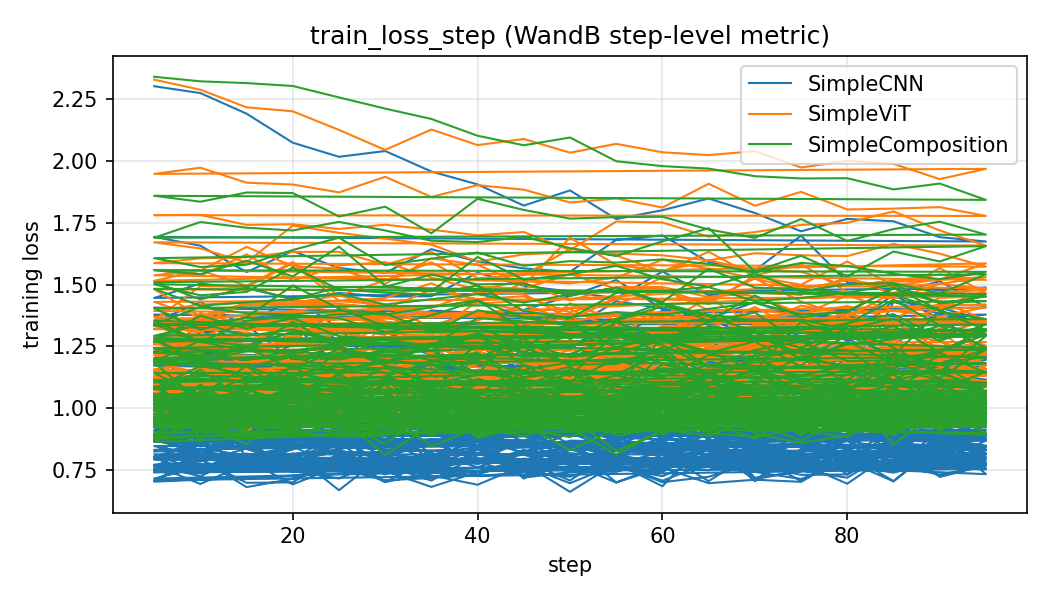
\includegraphics[width=0.72\linewidth]{fig_metric_train_loss_step.png}
  \caption{W\&B \texttt{train\_loss\_step}: the CNN descends fastest to the lowest loss; the ViT plateaus higher; the Composition lies between.}
  \label{fig:step}
\end{figure}

\begin{figure}[ht!]\centering
  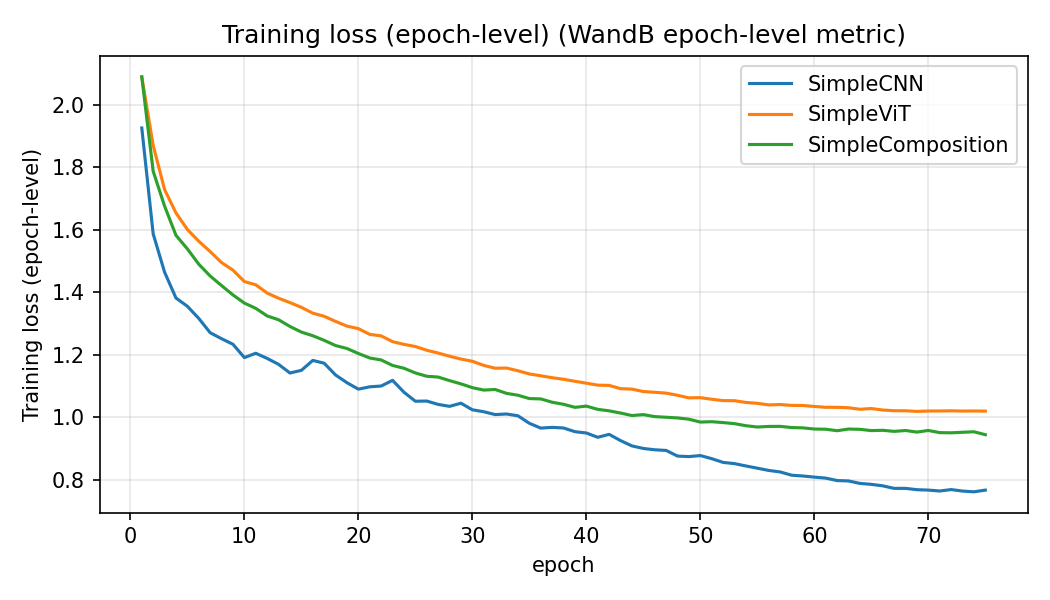
\includegraphics[width=0.72\linewidth]{fig_metric_train_loss_epoch.png}
  \caption{W\&B \texttt{train\_loss\_epoch}: the ViT leaves more training loss, i.e.\ it underfits this small-data task without convolutional inductive bias.}
  \label{fig:loss}
\end{figure}

\begin{figure}[ht!]\centering
  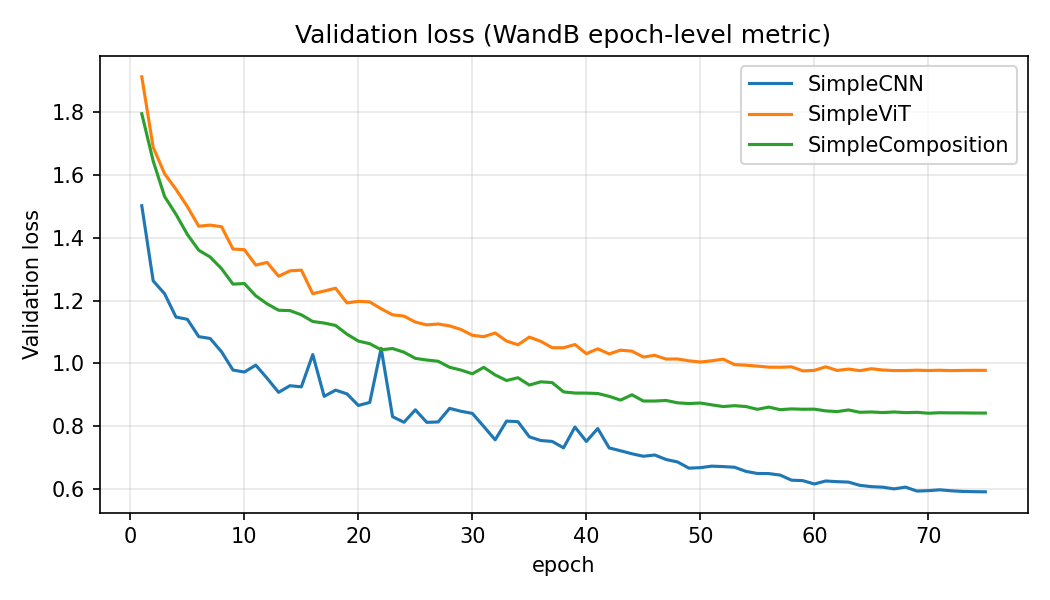
\includegraphics[width=0.72\linewidth]{fig_metric_val_loss.png}
  \caption{W\&B \texttt{val\_loss}: the CNN generalises best; the ViT's higher loss is consistent with the expected weakness of Transformers on small datasets.}
  \label{fig:vloss}
\end{figure}

\begin{figure}[ht!]\centering
  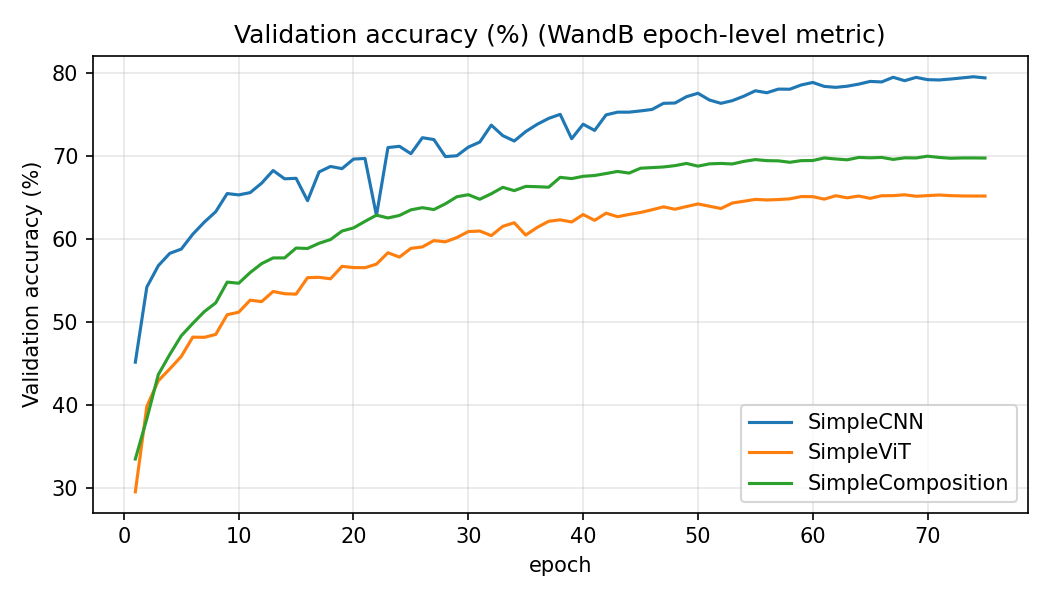
\includegraphics[width=0.72\linewidth]{fig_metric_val_acc.png}
  \caption{W\&B \texttt{val\_acc}: CNN vs.\ ViT vs.\ Composition on one axis. The CNN reaches $79.54\%$ and is still improving when the cosine schedule ends, whereas the ViT saturates near $65.2\%$.}
  \label{fig:acc}
\end{figure}

The four W\&B metrics above (step loss, epoch loss, validation loss, validation accuracy) show a consistent picture: the CNN converges fastest and best, the plain ViT saturates early, and the Composition recovers part of the gap. This matches the handout's remark that removing the convolutional inductive bias hurts in the small-data/small-model regime. Final test accuracies: \textbf{CNN 79.48\%}, \textbf{ViT 65.01\%}, \textbf{Composition 69.98\%}.

\section{Bonus: SimpleComposition}
\texttt{SimpleComposition} feeds the CNN feature maps (\texttt{forward\_map}, $32\times4\times4$) into a small ViT ($patch=2\times2$, $dim=64$, $depth=2$) and trains end-to-end. Under the course counting rule (CNN non-linear part + full ViT) it uses $5{,}088+76{,}106=81{,}194<120$K parameters and reaches \textbf{69.98\%} test accuracy (curve in \cref{fig:acc}), clearly above the plain ViT.

\section{Conclusion}
The compact CNN gives the best accuracy/size trade-off, the from-scratch ViT is limited by the small-data regime, and a CNN--ViT composition partially closes the gap. All runs are reproducible (fixed seeds, saved hyper-parameters, W\&B logging).

\bibliographystyle{plainnat}
\bibliography{reference}
\end{document}
